\documentclass{standalone}
\usepackage{tikz}
\usepackage{ctex,siunitx,ninecolors}
\setCJKmainfont{Noto Serif CJK SC}
\usepackage{tkz-euclide}
\usepackage{amsmath}
\usetikzlibrary{patterns, calc}
\usetikzlibrary {decorations.pathmorphing, decorations.pathreplacing, decorations.shapes,}
\begin{document}
\small
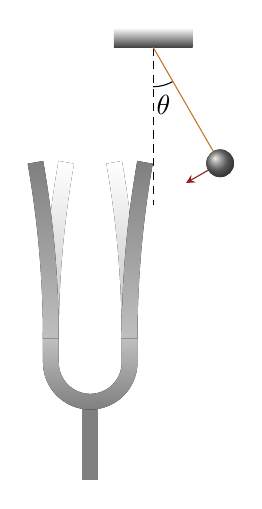
\begin{tikzpicture}[>=stealth, scale=1.0]
  % \useasboundingbox(-0.5,1.34)rectangle(7.55,-1.47);
  \begin{scope}[yshift=-4cm,xshift=-0.8cm]
    \fill[gray](0.1,-0.45)rectangle(-0.1,-1.5);
    \fill[top color=lightgray,bottom color=gray](-0.4,0)arc(180:360:0.4)--++(0,0.3)--++(0.2,0)--++(0,-0.3)arc(0:-180:0.6)--++(0,0.3)--++(0.2,0)--cycle;
    \fill[bottom color=lightgray,top color=white](0.6,0.3)arc(0:10:13)--++(190:0.2)arc(10:0:12.8);
    \fill[bottom color=lightgray,top color=white](-0.4,0.3)arc(180:170:12.8)--++(170:0.2)arc(170:180:13);
    \fill[bottom color=lightgray,top color=gray](-0.4,0.3)arc(0:10:13)--++(190:0.2)arc(10:0:12.8);
    \fill[bottom color=lightgray,top color=gray](0.6,0.3)arc(180:170:12.8)--++(170:0.2)arc(170:180:13);
  \end{scope}
  \fill[bottom color=darkgray,top color=white](-0.5,0)rectangle(0.5,0.25);
  \draw[densely dashed](0,0)--(0,-2.0);
  \draw[thin](0,-0.5)arc(-90:-60:0.5)node[midway,below]{$\theta$};
  \draw[brown6](0,0)--(-60:1.7);
  \draw[->,red3](-60:1.7)--++(210:0.5);
  \fill[ball color=gray](-60:1.7)circle(5pt);
\end{tikzpicture}
\end{document}
